\textbf{What is the right mix of power sources?} To understand the behavior of the proposed tool, we carry out 5 settings in practice. For each setting, the data center use different mixes of PV, GE, and Grid. As shown in Table~\ref{tbl:right_mix}, the right mix of power sources are under different scenarios. Setting 1 requires all 3 sources of power while other settings neglect some of power sources. For example, GE will not be planned if the gas price is very high as setting 2. In setting 3, it not necessary to import electricity from the public electrical grid because the capacity of GE generators is fixed and data center prefer PV generation to the electricity from the public grid. Setting 4 shows that the data center only provision the PV generation and public grid if the gas prices are equivalent to the electricity prices. When the gas price is cheap and has the GE capacity available, the data center operators should go with only the GE generation.

\begin{table}[!ht]
	\centering
	\caption{Right mix of power sources under different scenarios.}	
	\begin{tabular}{|p{0.5cm}|p{1cm}|p{1.2cm}|p{1cm}|p{2cm}|}
		\hline
		No. & Gas price (\$/kWh) & GE capacity range (kW) & Utility tariff (\$/kWh) & Power sources \\ \hline \hline
		1 & 0.07 & [0,1400] & 0.08 & PV+GE+Grid \\  \hline
		2 & 0.14 & [0,1400] & 0.08 & PV+Grid    \\  \hline
		3 & 0.07 & 633      & 0.08 & PV+GE      \\  \hline
		4 & 0.03 & [0,1400] & 0.03 & PV+Grid    \\  \hline
		5 & 0.03 & 633      & 0.08 & GE only    \\  \hline
	\end{tabular}
	\label{tbl:right_mix}
\end{table}


\emph{Consolidation level: } The level of consolidation indicates the maximum utilization of servers in a data center to serve workload. We assume that the interactive workload occupies 40\% utilization of servers. Hence, we start evaluating consolidation level from 0.4 which is the minimum level to serve the remaining flexible workload. Figure~\ref{f.capacity_con} shows that the capacities of PV and Grid slightly go up and down as the consolation level increase, which is opposite to the change of GE capacity. Although the consolidation level does not strongly affect the capacities, it still reduce the O\&M expenditure as shown in Figure~\ref{f.cost_con}.

%\begin{enumerate}
%\item PV capacity first increases, then decreases.
%\item With higher utilization, the total cost decreases\end{enumerate}

%TCO_grid_payback_con.m
\begin{figure}[!ht]
	\begin{center}
		\subfigure[Capacity]{{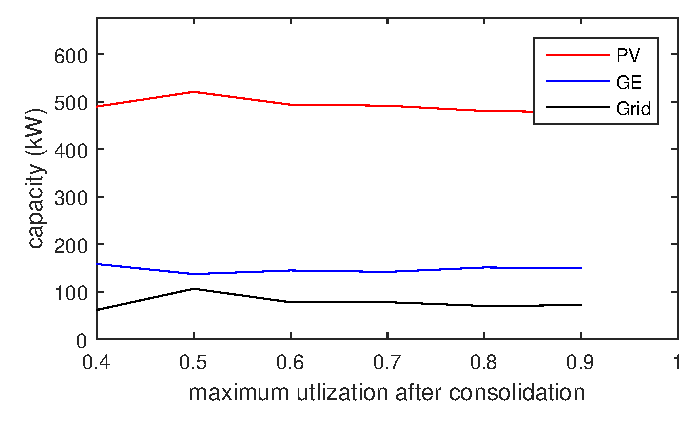
\includegraphics[width=0.48\columnwidth]{figs/capacity_con}}
			\label{f.capacity_con}}
		\subfigure[Cost]{{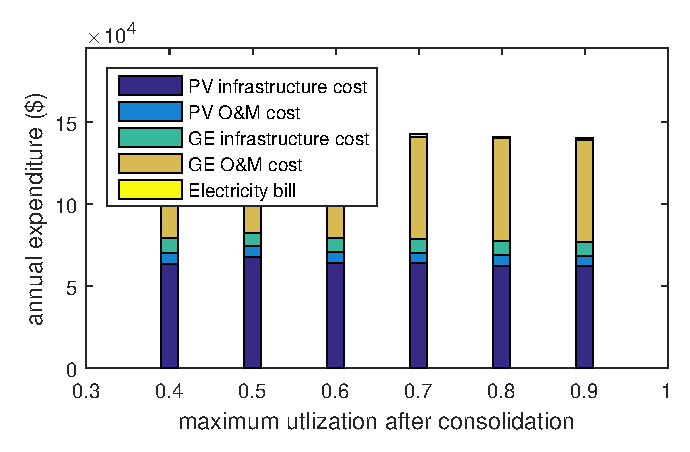
\includegraphics[width=0.48\columnwidth]{figs/cost_con}}
			\label{f.cost_con}}
		\caption{Impact of different consolidation levels.}
		\label{f.consolidation}
	\end{center}
\end{figure}